\section{Learning Deformable 3D Models}
\seclabel{modelLearning}

\begin{figure*}[htb!]
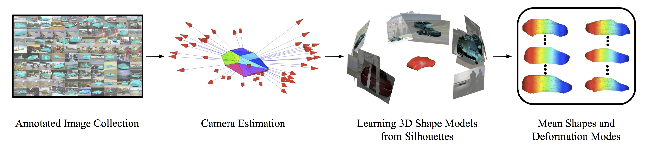
\includegraphics[width = \textwidth]{figures/categoryshapes/figTrain.pdf}
\caption{Overview of our training pipeline. We use an annotated image collection to estimate camera projection parameters which we then use along with object silhouettes to learn 3D shape models. Our learnt shape models, as illustrated in the rightmost figure are capable of deforming to capture intra-class shape variation.}
\label{fig:figtrain}
\end{figure*}

We are interested in learning 3D shape models that can be robustly aligned to noisy object segmentations by incorporating top-down class-specific knowledge of how shapes from the class typically project onto the image. We want to learn such models from just 2D training images, aided by ground truth segmentations and a few keypoints, similar to \cite{carvi14}. Our approach operates by first estimating the projection parameters (camera) for all objects in a class using a structure-from-motion approach, followed by optimizing over a deformation basis of representative 3D shapes that best explain all silhouettes, conditioned on the estimated cameras. We describe these two stages of model learning in the following subsections. Figure \ref{fig:figtrain} illustrates this training pipeline of ours.

\subsection{Camera Estimation}
\seclabel{nrsfm}
We use the framework of NRSfM \cite{Bregler2000} to jointly estimate the projection parameters (rotation, translation and scale) for all training instances in each class. Originally proposed for recovering shape and deformations from video \cite{nrsfm_priors,Torresani2008NRSFM,varnrsfm2013,Bregler2000}, NRSfM is a natural choice for camera estimation from sparse correspondences as intra-class variation may become a confounding factor if not modeled explicitly. However, the performance of such algorithms has only been explored on simple categories, such as SUV's \cite{Zhu_ModelEvolution:2010} or flower petal and clown fish \cite{prasad2010finding}. Closer to our work, Hejrati and Ramanan \cite{HejratiR12} used NRSfM on a larger class (cars) but need a predictive detector to fill-in missing data (occluded keypoints) which we do not assume to have here.

%To cope with the highly under-constrained nature of the problem most methods have dwelled on low-rank factorizations of the shape matrix \cite{Bregler2000,Brand2005}, or on imposing priors on shapes and deformations \cite{Torresani2008NRSFM,nrsfm_priors,varnrsfm2013}. }

We closely follow the EM-PPCA formulation of Torresani \etal\cite{Torresani2008NRSFM} and propose a simple extension to the algorithm that incorporates silhouette information in addition to keypoint correspondences to robustly recover cameras and shape bases. Energies similar to ours have been proposed in the shape-from-silhouette  \cite{balloonshapes} and rigid structure-from-motion \cite{carvi14} literature but, to the best of our knowledge, not in conjunction with NRSfM.

\vspace{3mm}
\noindent \textbf{NRSfM Model Formulation.} We are provided with an annotated training set $T:\{(O_n, P_n)\}_{n=1}^N$, where $O_n$ is the instance silhouette and $P_n \in \mathbb{R}^{2 \times K}$ denotes the annotated keypoint coordinates, possibly with missing entries (occluded/truncated keypoints). The annotated keypoints $P_n$ are  projections of the underlying 3D points $W_n \in \mathbb{R}^{3 \times K}$ via the projection function $\pi_n$. In the \nrsfm model, the space of 3D keypoint locations $W_n$ is parametrized linearly and the projection function is assumed to be weakly orthographic \ie $\pi_n \equiv (c_n, R_n, T_n)$, where $c_n$ represents scale, $R_n \in \mathbb{R}^{2 \times 3}$ denotes rotation and $T_n \in \mathbb{R}^{1 \times 2}$ corresponds to 2D translation. Our goal is to infer the camera parameters $(c_n, R_n, T_n)$ as well as 3D keypoint locations $W_n$ for all instances in the annotated training set.

Formally, our adaptation of the \nrsfm algorithm in \cite{Torresani2008NRSFM} corresponds to maximizing the likelihood of the following model:

\begin{equation}
\begin{aligned}
&{P_{n}} = c_nR_nW_{n} + 1^TT_{n} + N_{n}\\
&W_n = \bar{W} + \sum\limits_{k=1}^B U_b z_{nb} \\
&z_n \sim \mathcal{N}(0,I), \quad N^k_{n}\sim \mathcal{N}(0,\sigma^2 I)
\end{aligned}
\end{equation}
\begin{align}
\text{subject to:}\nonumber &\quad R_nR_{n}^{T} = I_2 \\
%\quad \forall n\in \{1,\cdots,N\}
\eqlabel{sil_constraint}
\sum\limits_{k=1}^K C_{n}^{mask}(p_{k,n}) &= 0, \quad \forall n\in \{1,\cdots,N\}
\end{align}

Here, the (partially) observed keypoint locations $P_n$ are assumed to be the projection under $\pi_n \equiv (c_n, R_n, T_n)$ of the 3D shape $W_n$ with white noise $N_n$. The shape is parameterized as a factored Gaussian with a mean shape $\bar{W}$, $B$ basis vectors $[U_1,U_2, \cdots,U_B] = U$ and latent deformation parameters $z_n$. Our key modification is constraint in \eqref{sil_constraint} where $C_{n}^{mask}$ denotes the Chamfer distance field of the $n^{th}$ instance's binary mask and says that all keypoints $p_{k,n}$ of instance $n$ should lie inside its binary mask. We observed that this results in more accurate cameras as well as more meaningful shape bases learnt from the data.

\vspace{3mm}
\noindent \textbf{Learning.} The likelihood of the above model is maximized using the EM algorithm. Missing data (occluded keypoints) is dealt with by ``filling-in" the values using the forward equations after the E-step. The algorithm computes shape parameters $\{\bar{W},U\}$, rigid body transformations $\{c_n,R_n,T_n\}$ as well as the deformation parameters $\{z_n\}$ for each training instance $n$. In practice, we augment the data using horizontally mirrored images to exploit bilateral symmetry in the object classes considered. We also precompute the Chamfer distance fields for the whole set to speed up computation. As shown in \figref{nrsfm_images}, \nrsfm  allows us to reliably predict cameras while being robust to intraclass variations.

\begin{figure}[htb!]
  \centering
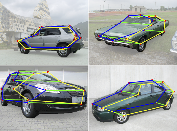
\includegraphics[width=.8\linewidth]{figures/categoryshapes/NRSFMCars.pdf}
\caption{NRSfM camera estimation: Estimated cameras visualized using a 3D car wireframe.}
\figlabel{nrsfm_images}
\end{figure}


%\label{densemodels}
Equipped with camera projection parameters and keypoint correspondences (now lifted to 3D by \nrsfm) on the whole training set, we proceed to build morphable 3D models for object categories from our major source of information in this paper - object silhouettes. This problem of reconstructing the 3D shape of a single object from its projected silhouettes in multiple calibrated images has been widely studied in the computer vision literature. Two prominent approaches are \textit{visual hulls} \cite{laurentini1994hull} and variational methods derived from \textit{snakes} e.g \cite{esteban2004snake,yusuf2006snake} which deform a surface mesh iteratively until convergence. Some recent papers have also extended variational approaches to the case of category shape reconstruction \cite{cashman2013dolphins,chen20123d}. While demonstrating accurate results on a limited number of categories, they typically require some form of 3D annotations to bootstrap the model and are computationally expensive. A recent work \cite{carvi14} has proposed a visual-hull based data-driven approach for class-based reconstruction for the first time on challenging real world datasets like PASCAL VOC. In contrast, we build parametric shape models for categories that compactly capture intra class shape variations. The benefits of having a model of 3D shape are manifold: 1) we are more robust to noisy inputs (silhouettes and pose) allowing us to pursue reconstruction in a fully automatic setting and 2) we forego the need for having continuous access to a large corpus of data. \RED{add points here.}

We propose an algorithm to learn class-specific 3D shape models given silhouette information and camera viewpoints estimated in the previous section. Our shape models inherently capture the intraclass variations in object categories and can be used to recover a 3D shape given an object's approximate silhouette and viewpoint in a new image.


\subsection{3D Basis Shape Model Learning}
\seclabel{basisshapes}
Equipped with camera projection parameters and keypoint correspondences (lifted to 3D by NRSfM) on the whole training set, we proceed to build deformable 3D shape models from object silhouettes within the same class. 3D shape reconstruction from multiple silhouettes projected from a single object in calibrated settings has been widely studied. Two prominent approaches are \textit{visual hulls} \cite{laurentini1994hull} and variational methods derived from \textit{snakes} e.g \cite{esteban2004snake,yusuf2006snake} which deform a surface mesh iteratively until convergence. Some interesting recent papers have extended variational approaches to handle categories \cite{cashman2013dolphins,chen20123d} but typically require some form of 3D annotations to bootstrap models. A recently proposed visual-hull based approach \cite{carvi14} requires only 2D annotations as we do for class-based reconstruction and it was successfully demonstrated on PASCAL VOC but does not serve our purpose as it makes strong assumptions about the accuracy of the segmentation and will in fact fill entirely any segmentation with a voxel layer. In contrast, we build parametric shape models for categories that compactly capture intra class shape variations. The benefits of having a model of 3D shape are manifold: 1) we are more robust to noisy inputs (silhouettes and pose) allowing us to pursue reconstruction in a fully automatic setting and 2) we can potentially sample novel shapes from an object category.

%We propose an algorithm to learn class-specific 3D shape models given silhouette information and camera viewpoints estimated in the previous section. Our shape models inherently capture the intraclass variations in object categories and can be used to recover a 3D shape given an object's approximate silhouette and viewpoint in a new image.

\paragraph{Shape Model Formulation.} We model our category shapes as a deformable point cloud - one per object class. As in the \nrsfm model, we use a linear combination of basis vectors to model these deformations. Note that we learn such models from silhouettes and this is what enables us to learn deformable models without relying on point correspondences between scanned 3D exemplars~\cite{blanz2003face}.

%In order to capture the intra-class variations using a single shape model, we must incorporate possible deformations. Similar to the NRSfM approach, the deformations we allow are a linear combination of  deformation bases. This setup, while using a formulation similar to NRSfM is significantly different because we do not assume any known correspondences or annotated points across images and the shape models we aim to infer are much denser (because of the large number of points in the representation).

The annotated training set $T:\{(O_n, P_n)\}_{n=1}^N$, where $O_n$ is the instance silhouette and $P_n \in \mathbb{R}^{2 \times K}$ denotes the annotated keypoint coordinates, is augmented after \nrsfm to contain $\pi_n$ (the projection function from world to image coordinates) and $W_n$ (3D coordinates for a small set of keypoints).
Our shape model $M = (\overline{S},V)$ comprises of a mean shape $\overline{S}$ and deformation bases $V = \{ V_1,.,V_K \} $ learnt from the augmented training set $T:\{(O_n,\pi_n, W_n)\}_{n=1}^N$. Note that the $\pi_i$ we obtain using NRSfM corresponds to orthographic projection but our algorithm could handle perspective projection as well.

In addition to the above, we use the following notations  --  $\pi(S)$ corresponds to the 2D projection of shape $S$, $C^{mask}$ refers to the Chamfer distance field of the binary mask of silhouette $O$ and $\Delta^k(p;Q)$ is defined as the squared average distance of point $p$ to its $k$ nearest neighbors in set $Q$.

\paragraph{Energy Formulation.} We formulate our objective function primarily based on image silhouettes. For example, the shape for an instance should always project within its silhouette and should agree with the keypoints (lifted to 3D by \nrsfm). We capture these by defining corresponding energy terms as follows:


\paragraph{Silhouette Consistency.} Silhouette consistency simply enforces the predicted shape for an instance to project inside its silhouette. This can be achieved by penalizing the points projected outside the instance mask by their distance from the silhouette (\ie squared distance to the closest silhouette point). In our $\Delta$ notation it can be written as follows:
\begin{gather}
 \label{eq:sil_con}E_{s}(S,O,\pi)=\underset{C^{mask}(p)>0}{\sum}\Delta^1(p;O)
\end{gather}


\paragraph{Silhouette Coverage.}
Using silhouette consistency alone would just drive points projected outside in towards the silhouette. This wouldn't ensure though that the object silhouette is ``filled'' - i.e. there might be overcarving. We deal with it by having an energy term that encourages points on the silhouette to pull nearby projected points towards them. Formally, this can be expressed as:
\begin{gather}
    \label{eq:sil_cov}E_{c}(S,O,\pi)=\underset{p\in O}{\sum}\Delta^m(p;\pi(S))
\end{gather}


\paragraph{Keypoint Consistency.} Our \nrsfm algorithm provides us with sparse 3D keypoints along with camera projection parameters. We use these sparse correspondences on the training set to deform the shape to explain these 3D points. The corresponding energy term penalizes deviation of the shape from the 3D keypoints $W$ for each instance. Specifically, this can be written as:
\begin{gather}
    \label{eq:kpgrad}E_{kp}(S,W)=\underset{\kappa\in W}{\sum}\Delta^m(\kappa;S)
\end{gather}


\paragraph{Local Consistency.} In addition to the above data terms, we use a simple shape regularizer to restrict arbitrary deformations by imposing a quadratic deformation penalty between every point and its neighbors. We also impose a similar penalty on deformations to ensure local smoothness. The $\delta$ parameter represents the mean squared displacement between neighboring points and it encourages all faces to have similar size. Here $V_{ki}$ is the $i^{th}$ point in the $k^{th}$ basis.
\begin{gather}
 \label{eq:local_con}E_{l}(\bar{S},V)=\underset{i}{\sum}\underset{j\in N(i)}{\sum}((\|\bar{S}_{i}-\bar{S}_{j}\| - \delta)^2 + \underset{k}{\sum}\|V_{ki}-V_{kj}\|^2)
 \end{gather}
 

\paragraph{Normal Smoothness.} Shapes occurring in the natural world tend to be locally smooth. We capture this prior on shapes by placing a cost on the variation of normal directions in a local neighborhood in the shape. Our normal smoothness energy is formulated as
\begin{gather}
 \label{eq:normal_con}E_{n}(S)=\underset{i}{\sum}\underset{j\in N(i)}{\sum}(1-\vec{\mathcal{N}_i} \cdot \vec{\mathcal{N}_j})
\end{gather}
 Here, $\vec{\mathcal{N}_i}$ represents the normal for the $i^{th}$ point in shape $S$ which is computed by fitting planes to local point neighborhoods. Our prior essentially states that local point neighborhoods should be flat. Note that this, in conjunction with our previous energies automatically enforces the commonly used prior that normals should be perpendicular to the viewing direction at the occluding contour~\cite{Barron2012B}.

Our total energy is given in equation \eqref{formulation}. In addition to the above smoothness priors we also penalize the $L_2$ norm of the deformation parameters $\alpha_i$ to prevent unnaturally large deformations.
\begin{gather}
\eqlabel{formulation}
E_{tot}(\bar{S},V,\alpha) = E_{l}(\bar{S},V)+\underset{i}{\sum}(E_{s}^i+E_{kp}^i+E_{c}^i+E_{n}^i+\underset{k}{\sum}(\|\alpha_{ik}V_k\|_F^{2}))
\end{gather}


\paragraph{Learning.} We solve the optimization problem in equation~\eqref{optimization} to obtain our shape model $M=(\bar{S},V)$. The mean shape and deformation basis are inferred via block-coordinate descent on $(\bar{S},V)$ and $\alpha$ using sub-gradient computations over the training set. We restrict $\|V_k\|_F$ to be a constant to address the scale ambiguity between $V$ and $\alpha$ in our formulation. In order to deal with imperfect segmentations and wrongly estimated keypoints, we use truncated versions of the above energies that reduce the impact of outliers. The mean shapes learnt using our algorithm for 9 rigid categories in PASCAL VOC are shown in Figure \ref{fig:meanDense}. Note that in addition to representing the coarse shape details of a category, the model also learns finer structures like chair legs and bicycle handles, which become more prominent with deformations.

\begin{equation}
\begin{aligned}
\eqlabel{optimization}
& \underset{\bar{S},V,\alpha}{\text{min}}
& & E_{tot}(\bar{S},V,\alpha) \\
& \text{subject to:}
& & S^i = \bar{S} + \underset{k}{\sum}\alpha_{ik} V_k
\end{aligned}
\end{equation}

Our training objective is highly non-convex and  non-smooth and is susceptible to initialization. We follow the suggestion of \cite{esteban2004snake} and initialize our mean shape with a soft visual hull computed using all training instances. The deformation bases and deformation weights are initialized randomly. 


\paragraph{Implementation Details.}
The gradients involved in our optimization for shape and projection parameters are extremely efficient to compute. We use approximate nearest neighbors computed using k-d tree to implement silhouette coverage,  keypoint consistency gradients and leverage Chamfer distance fields for obtaining silhouette consistency gradients. Our overall computation takes only about 15 min to learn a deformable shape model for an object category with about 500 annotated examples.

\begin{figure}[htb!]
\centering
  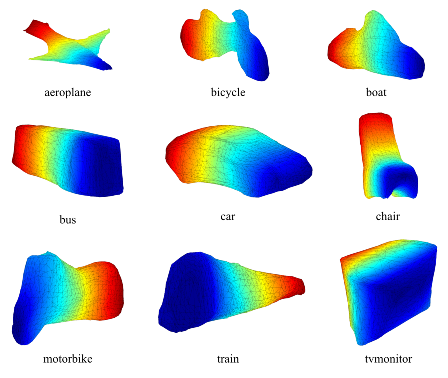
\includegraphics[width=\textwidth]{figures/categoryshapes/meanShapesCrop.pdf}
  \caption{Mean shapes learnt for rigid classes in PASCAL VOC obtained using our basis shape formulation. Color encodes depth when viewed frontally.}
  \label{fig:meanDense}
\end{figure}

